\documentclass{standalone}
\usepackage{tikz}
\usetikzlibrary{patterns, positioning}


\begin{document}
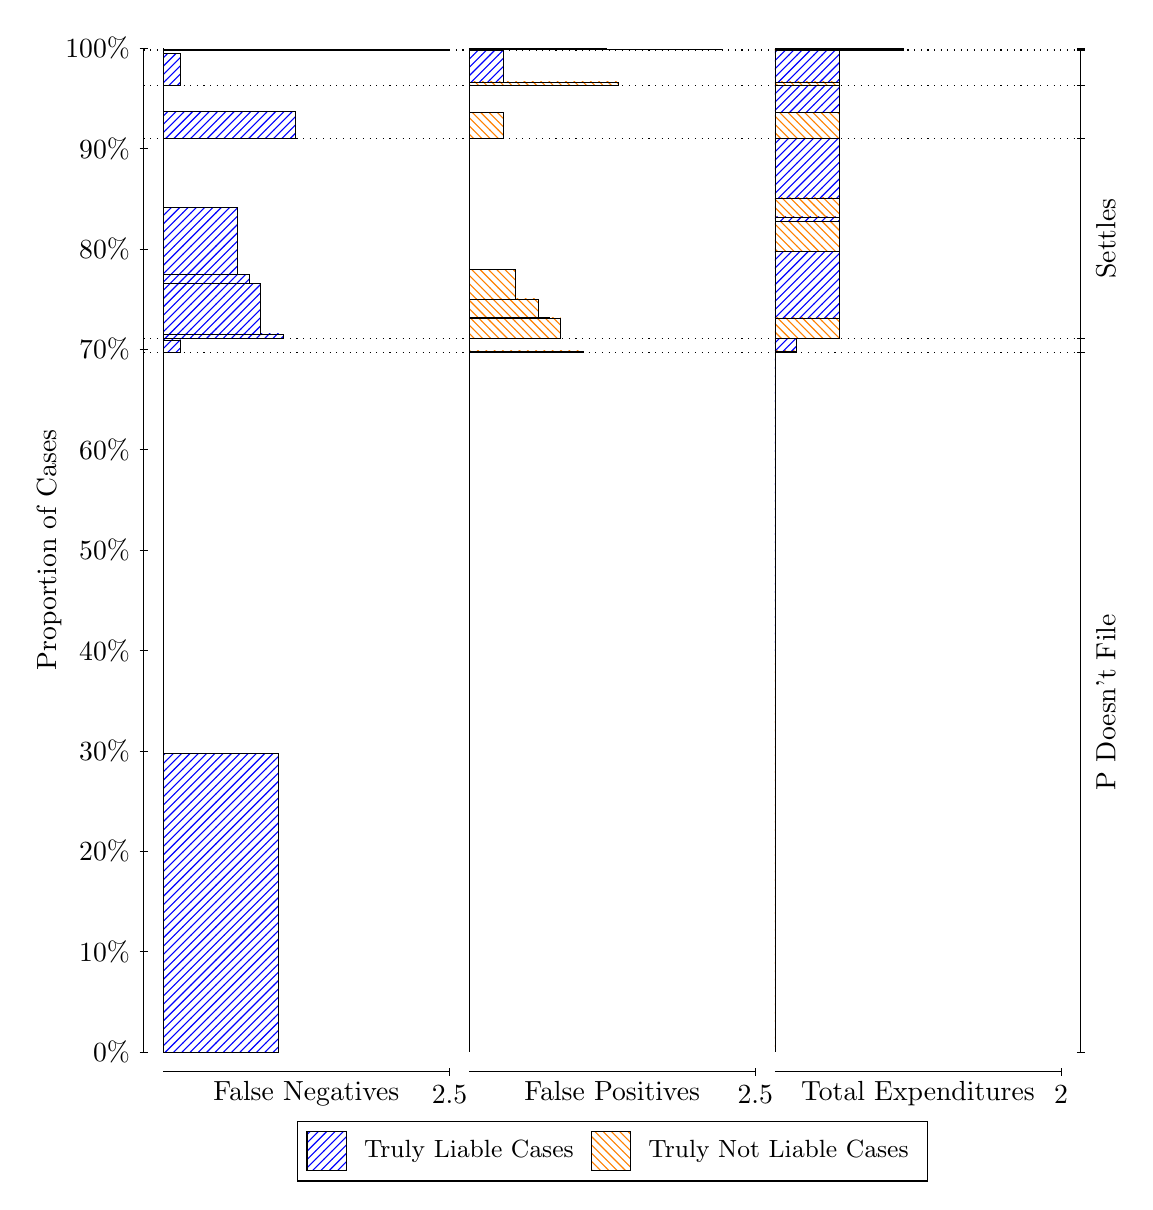
\begin{tikzpicture}
\draw[black, very thin] (1.5,1.75) -- (1.5,14.5);
\node[rotate=90, text=black, anchor=center] at (0.3, 8.125) {Proportion of Cases};
\draw[black, very thin] (1.45,1.75) -- (1.55,1.75);
\node[text=black, anchor=east] at (1.45, 1.75) {0\%};
\draw[black, very thin] (1.45,3.025) -- (1.55,3.025);
\node[text=black, anchor=east] at (1.45, 3.025) {10\%};
\draw[black, very thin] (1.45,4.3) -- (1.55,4.3);
\node[text=black, anchor=east] at (1.45, 4.3) {20\%};
\draw[black, very thin] (1.45,5.575) -- (1.55,5.575);
\node[text=black, anchor=east] at (1.45, 5.575) {30\%};
\draw[black, very thin] (1.45,6.85) -- (1.55,6.85);
\node[text=black, anchor=east] at (1.45, 6.85) {40\%};
\draw[black, very thin] (1.45,8.125) -- (1.55,8.125);
\node[text=black, anchor=east] at (1.45, 8.125) {50\%};
\draw[black, very thin] (1.45,9.4) -- (1.55,9.4);
\node[text=black, anchor=east] at (1.45, 9.4) {60\%};
\draw[black, very thin] (1.45,10.675) -- (1.55,10.675);
\node[text=black, anchor=east] at (1.45, 10.675) {70\%};
\draw[black, very thin] (1.45,11.95) -- (1.55,11.95);
\node[text=black, anchor=east] at (1.45, 11.95) {80\%};
\draw[black, very thin] (1.45,13.225) -- (1.55,13.225);
\node[text=black, anchor=east] at (1.45, 13.225) {90\%};
\draw[black, very thin] (1.45,14.5) -- (1.55,14.5);
\node[text=black, anchor=east] at (1.45, 14.5) {100\%};

\draw[black, very thin] (13.4,1.75) -- (13.4,14.5);
\draw[black, very thin] (13.35,1.75) -- (13.45,1.75);
\node[anchor=west] at (13.35, 1.75) {};
\draw[black, very thin] (13.35,10.636) -- (13.45,10.636);
\node[anchor=west] at (13.35, 10.636) {};
\draw[black, very thin] (13.35,10.811) -- (13.45,10.811);
\node[anchor=west] at (13.35, 10.811) {};
\draw[black, very thin] (13.35,13.354) -- (13.45,13.354);
\node[anchor=west] at (13.35, 13.354) {};
\draw[black, very thin] (13.35,14.027) -- (13.45,14.027);
\node[anchor=west] at (13.35, 14.027) {};
\draw[black, very thin] (13.35,14.474) -- (13.45,14.474);
\node[anchor=west] at (13.35, 14.474) {};
\draw[black, very thin] (13.35,14.482) -- (13.45,14.482);
\node[anchor=west] at (13.35, 14.482) {};
\draw[black, very thin] (13.35,14.5) -- (13.45,14.5);
\node[anchor=west] at (13.35, 14.5) {};

\draw[black, very thin, pattern color=blue, pattern=north east lines] (1.75,1.75) rectangle (3.2033,5.5421);
\draw[black, very thin, pattern color=orange, pattern=north west lines] (1.75,5.5421) rectangle (1.75,10.636);
\draw[black, very thin, pattern color=blue, pattern=north east lines] (1.75,10.636) rectangle (1.968,10.793);
\draw[black, very thin, pattern color=orange, pattern=north west lines] (1.75,10.793) rectangle (1.75,10.811);
\draw[black, very thin, pattern color=blue, pattern=north east lines] (1.75,10.811) rectangle (3.276,10.87);
\draw[black, very thin, pattern color=blue, pattern=north east lines] (1.75,10.87) rectangle (2.9853,11.51);
\draw[black, very thin, pattern color=blue, pattern=north east lines] (1.75,11.51) rectangle (2.84,11.627);
\draw[black, very thin, pattern color=blue, pattern=north east lines] (1.75,11.627) rectangle (2.6947,12.473);
\draw[black, very thin, pattern color=orange, pattern=north west lines] (1.75,12.473) rectangle (1.75,13.354);
\draw[black, very thin, pattern color=blue, pattern=north east lines] (1.75,13.354) rectangle (3.4213,13.695);
\draw[black, very thin, pattern color=orange, pattern=north west lines] (1.75,13.695) rectangle (1.75,14.027);
\draw[black, very thin, pattern color=blue, pattern=north east lines] (1.75,14.027) rectangle (1.968,14.431);
\draw[black, very thin, pattern color=orange, pattern=north west lines] (1.75,14.431) rectangle (1.75,14.474);
\draw[black, very thin, pattern color=blue, pattern=north east lines] (1.75,14.474) rectangle (5.3833,14.478);
\draw[black, very thin, pattern color=orange, pattern=north west lines] (1.75,14.478) rectangle (1.75,14.482);
\draw[black, very thin, pattern color=orange, pattern=north west lines] (1.75,14.482) rectangle (1.75,14.486);
\draw[black, very thin, pattern color=blue, pattern=north east lines] (1.75,14.486) rectangle (1.75,14.5);
\draw[black, very thin, pattern color=orange, pattern=north west lines] (5.6333,1.75) rectangle (5.6333,6.8434);
\draw[black, very thin, pattern color=blue, pattern=north east lines] (5.6333,6.8434) rectangle (5.6333,10.636);
\draw[black, very thin, pattern color=orange, pattern=north west lines] (5.6333,10.636) rectangle (7.0867,10.653);
\draw[black, very thin, pattern color=blue, pattern=north east lines] (5.6333,10.653) rectangle (5.6333,10.811);
\draw[black, very thin, pattern color=orange, pattern=north west lines] (5.6333,10.811) rectangle (6.796,11.072);
\draw[black, very thin, pattern color=orange, pattern=north west lines] (5.6333,11.072) rectangle (6.6507,11.083);
\draw[black, very thin, pattern color=orange, pattern=north west lines] (5.6333,11.083) rectangle (6.5053,11.314);
\draw[black, very thin, pattern color=orange, pattern=north west lines] (5.6333,11.314) rectangle (6.2147,11.691);
\draw[black, very thin, pattern color=blue, pattern=north east lines] (5.6333,11.691) rectangle (5.6333,13.354);
\draw[black, very thin, pattern color=orange, pattern=north west lines] (5.6333,13.354) rectangle (6.0693,13.686);
\draw[black, very thin, pattern color=blue, pattern=north east lines] (5.6333,13.686) rectangle (5.6333,14.027);
\draw[black, very thin, pattern color=orange, pattern=north west lines] (5.6333,14.027) rectangle (7.5227,14.07);
\draw[black, very thin, pattern color=blue, pattern=north east lines] (5.6333,14.07) rectangle (6.0693,14.474);
\draw[black, very thin, pattern color=orange, pattern=north west lines] (5.6333,14.474) rectangle (5.6333,14.478);
\draw[black, very thin, pattern color=blue, pattern=north east lines] (5.6333,14.478) rectangle (5.6333,14.482);
\draw[black, very thin, pattern color=orange, pattern=north west lines] (5.6333,14.482) rectangle (8.8307,14.486);
\draw[black, very thin, pattern color=blue, pattern=north east lines] (5.6333,14.486) rectangle (7.3773,14.5);
\draw[black, very thin, pattern color=orange, pattern=north west lines] (9.5167,1.75) rectangle (9.5167,6.8434);
\draw[black, very thin, pattern color=blue, pattern=north east lines] (9.5167,6.8434) rectangle (9.5167,10.636);
\draw[black, very thin, pattern color=orange, pattern=north west lines] (9.5167,10.636) rectangle (9.7892,10.653);
\draw[black, very thin, pattern color=blue, pattern=north east lines] (9.5167,10.653) rectangle (9.7892,10.811);
\draw[black, very thin, pattern color=orange, pattern=north west lines] (9.5167,10.811) rectangle (10.334,11.072);
\draw[black, very thin, pattern color=blue, pattern=north east lines] (9.5167,11.072) rectangle (10.334,11.919);
\draw[black, very thin, pattern color=orange, pattern=north west lines] (9.5167,11.919) rectangle (10.334,12.296);
\draw[black, very thin, pattern color=blue, pattern=north east lines] (9.5167,12.296) rectangle (10.334,12.356);
\draw[black, very thin, pattern color=orange, pattern=north west lines] (9.5167,12.356) rectangle (10.334,12.597);
\draw[black, very thin, pattern color=blue, pattern=north east lines] (9.5167,12.597) rectangle (10.334,13.354);
\draw[black, very thin, pattern color=orange, pattern=north west lines] (9.5167,13.354) rectangle (10.334,13.686);
\draw[black, very thin, pattern color=blue, pattern=north east lines] (9.5167,13.686) rectangle (10.334,14.027);
\draw[black, very thin, pattern color=orange, pattern=north west lines] (9.5167,14.027) rectangle (10.334,14.07);
\draw[black, very thin, pattern color=blue, pattern=north east lines] (9.5167,14.07) rectangle (10.334,14.474);
\draw[black, very thin, pattern color=orange, pattern=north west lines] (9.5167,14.474) rectangle (11.152,14.478);
\draw[black, very thin, pattern color=blue, pattern=north east lines] (9.5167,14.478) rectangle (11.152,14.482);
\draw[black, very thin, pattern color=orange, pattern=north west lines] (9.5167,14.482) rectangle (11.152,14.486);
\draw[black, very thin, pattern color=blue, pattern=north east lines] (9.5167,14.486) rectangle (11.152,14.5);
\draw[black, dotted] (1.5,10.636) -- (13.4,10.636);
\draw[black, dotted] (1.5,10.811) -- (13.4,10.811);
\draw[black, dotted] (1.5,13.354) -- (13.4,13.354);
\draw[black, dotted] (1.5,14.027) -- (13.4,14.027);
\draw[black, dotted] (1.5,14.474) -- (13.4,14.474);
\draw[black, dotted] (1.5,14.482) -- (13.4,14.482);
\draw[black, very thin] (1.75,1.5) -- (5.3833,1.5);
\node[text=black, anchor=north] at (3.5667, 1.5) {False Negatives};
\draw[black, very thin] (5.3833,1.45) -- (5.3833,1.55);
\node[text=black, anchor=north] at (5.3833, 1.45) {2.5};

\draw[black, very thin] (5.6333,1.5) -- (9.2667,1.5);
\node[text=black, anchor=north] at (7.45, 1.5) {False Positives};
\draw[black, very thin] (9.2667,1.45) -- (9.2667,1.55);
\node[text=black, anchor=north] at (9.2667, 1.45) {2.5};

\draw[black, very thin] (9.5167,1.5) -- (13.15,1.5);
\node[text=black, anchor=north] at (11.333, 1.5) {Total Expenditures};
\draw[black, very thin] (13.15,1.45) -- (13.15,1.55);
\node[text=black, anchor=north] at (13.15, 1.45) {2};

\node[text=black, centered, rotate=90] at (13.72, 6.1928) {P Doesn't File};

\node[text=black, centered, rotate=90] at (13.72, 12.082) {Settles};





\draw (7.449999999999999,1.5) node[draw=none] (baseCoordinate) {};
\begin{scope}[align=center]
        \matrix[scale=0.5, draw=black, below=0.5cm of baseCoordinate, nodes={draw}, column sep=0.1cm]{
            \node[rectangle, draw, minimum width=0.5cm, minimum height=0.5cm, pattern color=blue, pattern=north east lines] {}; &
            \node[draw=none, font=\small, text=black] (B) {Truly Liable Cases}; &
            \node[rectangle, draw, minimum width=0.5cm, minimum height=0.5cm, pattern color=orange, pattern=north west lines] {}; &
            \node[draw=none, font=\small, text=black] (B) {Truly Not Liable Cases}; \\
            };
\end{scope}

\end{tikzpicture}
\end{document}